\documentclass[11pt]{article}
\usepackage[margin=1in]{geometry}
\usepackage[T1]{fontenc}
\usepackage{lmodern}
\usepackage{microtype}
\usepackage{amsmath,amssymb}
\usepackage{booktabs}
\usepackage{multirow}
\usepackage{enumitem}
\usepackage{xcolor}
\usepackage{pgfplots}
\pgfplotsset{compat=1.17}
\usepackage[colorlinks=true,linkcolor=blue!50!black,citecolor=blue!50!black,urlcolor=blue!50!black]{hyperref}
\setlist{itemsep=2pt}

\newcommand{\onepath}{one-path}
\newcommand{\status}[1]{\textsf{\small #1}}

\title{Commit, Solve, Sample:\\ Where Recursive Reasoners Fail on Problems with Many Answers\\[4pt]
\large Partial project report}
\author{Harshit Bisht}
\date{November 2026}

\begin{document}
\maketitle

\begin{abstract}
A reasoner facing a problem with several correct answers must pick one of them consistently, solve the problem, and,
for test-time scaling to pay off, be able to produce other answers when asked again. We study these three abilities
in tiny recursive reasoning models on two tasks whose solution sets are known exactly: 10$\times$10 N-Queens
completion and 15$\times$15 mazes with 1 to 924 shortest paths. We compare deterministic models trained naively or
with one-of-many objectives against GRAM, which adds a latent variable. Three findings so far. (1) Naive training
does not fail by averaging the solutions, as is commonly assumed. In one pass the model confidently follows
\emph{different} solutions in different parts of the output (N-Queens) or abstains at choice points (mazes).
Decoding one decision at a time and re-running the model after each lifts naive TRM from 37\% to 99.4\% on mazes,
the best single-answer result of any model we trained, and from 1\% to 78\% on N-Queens. (2) The remaining errors are
of a different kind: solver errors on inputs with a unique answer, where the training objective matters and its
effect depends on the domain (naive training is the best solver on unique mazes and the worst on unique N-Queens
boards). (3) Deterministic models pick their answer within the first one or two recursion steps, from the initial
latent state. Perturbing that state and the board's symmetries at test time gives them diversity without any
latent-variable training: on N-Queens this matches GRAM's coverage (99.5\% vs.\ 99.9\% of solutions in 100 samples)
with a better first sample (96.6\% vs.\ 91.0\%); on mazes it closes most but not all of the gap (54\% vs.\ 69\%
coverage, less even). Our original hypothesis, that GRAM's single KL weight forces a trade-off that a per-input KL
budget would fix, was largely refuted: longer training removed most of the trade-off and the budget failed.
\end{abstract}

\section{Problem}

Many problems we would like neural reasoners to solve have more than one correct answer: puzzles with several
completions, plans and routes with equal cost, proofs with different steps. Several abilities then matter, and they
can pull in different directions:
\begin{enumerate}[label=(\roman*)]
  \item \textbf{Consistency.} All parts of an answer must come from the \emph{same} solution. A model that is right
  about each part separately can still combine parts of different solutions into an invalid whole.
  \item \textbf{Reliability.} A single attempt should be correct, especially when the answer is unique and there is
  nothing to choose between.
  \item \textbf{Coverage.} Across attempts, the model should produce many different correct answers, ideally in
  proportion to how many exist. This is what makes test-time compute useful: majority voting, best-of-$n$ with a
  verifier, and meeting requirements that were not known at training time all need distinct correct candidates.
\end{enumerate}

The same tensions run through current work on reasoning in large language models.
\begin{itemize}
  \item \textbf{Self-consistency}~\cite{wang2023selfconsistency} votes over sampled solutions; it helps only if the
  samples are diverse and mostly correct.
  \item \textbf{Verifiers}~\cite{cobbe2021verifiers} pick the best of $n$ samples; they help only if some sample is
  correct.
  \item \textbf{Test-time scaling}~\cite{snell2024scaling,brown2024monkeys} spends more compute on sampling or
  revision; the return depends on how coverage grows with the number of samples.
  \item \textbf{RL with verifiable rewards} raises pass@1, and whether it also narrows the set of solutions the model
  can reach (lower pass@$k$ at large $k$) is debated~\cite{yue2025rl,wen2025rlvr}.
  \item \textbf{Parallel decoding} of several output positions at once mixes different valid outputs, the
  ``multimodality problem'' of non-autoregressive translation~\cite{gu2018nat}; masked diffusion models face the
  same issue and decode the most confident positions first~\cite{kim2025ordering}.
\end{itemize}
In LLMs these effects are hard to measure precisely, because the set of correct answers is neither known nor
enumerable. We study them where it is: recursive reasoning models on combinatorial tasks whose solution sets can be
counted exactly.

\paragraph{Models.} The Tiny Recursive Model (TRM)~\cite{jolicoeur2025trm}, a simplification of the Hierarchical
Reasoning Model~\cite{wang2025hrm}, refines a latent state by applying one small network repeatedly, with deep
supervision and learned halting. It is deterministic: one input gives one answer. It predicts every output cell at
once. Trained naively on all solutions of an input, it is said to average them and produce invalid
outputs~\cite{nandwani2021oneofmany}. One-of-many learning (1oML)~\cite{nandwani2021oneofmany} instead trains towards
one solution per input, chosen as the closest (\emph{MinLoss}) or sampled by model likelihood (\emph{I-ExplR}); two
simpler baselines train on one fixed random solution (\emph{Random}) or only on inputs with a unique solution
(\emph{Unique}). GRAM~\cite{baek2026gram} makes the recursion stochastic. At every recursion step it adds a latent
$z$ to the state, drawn during training from a posterior $q(z\mid x,y)$ that sees the target $y$, and at test time
from a prior $p(z\mid x)$. It is trained with an evidence lower bound whose KL term has one global weight $\beta$.

\paragraph{Research questions.} \emph{Why do recursive reasoners fail on inputs with many answers: at learning the
solutions, at decoding a consistent one, or at solving? And what does it take to get diverse, correct samples:
a latent variable trained for it, or is a deterministic model enough?}

\section{Hypotheses and how they fared}

We started from a hypothesis about GRAM (H1--H5 below, stated in our proposal). Results refuted or narrowed most of
them, and pointed to a different set of questions (D1--D3), which now organise the project.

\paragraph{Original hypotheses.} For a target drawn uniformly from an input's $k(x)$ solutions, a latent that
identifies the target needs about $\ln k(x)$ nats, but GRAM charges every input the same KL price $\beta$. We
expected: \textbf{H1}, a trade-off between single-sample accuracy on unique-answer inputs (low $\beta$ lets the
posterior leak the answer, so prior samples fail) and coverage on ambiguous ones (high $\beta$ collapses the latent),
that more training does not remove; \textbf{H2}, that charging KL only above a per-input budget $b\ln k(x)$ fixes
it; \textbf{H3}, that an estimated budget keeps most of the gain; \textbf{H4}, that diversity cannot be obtained
without a posterior; \textbf{H5}, that the halting head can rank samples like a verifier.

\begin{table}[h]
\centering\small
\begin{tabular}{@{}lp{11.5cm}@{}}
\toprule
& Outcome \\
\midrule
H1 & \textbf{Mostly refuted.} The trade-off exists at 50k steps, but at 100k steps $\beta=0.015$ reaches 91.3\% on one
sample (83.7\% on \onepath{} mazes) with unchanged coverage. The good range of $\beta$ is narrow (0.01 leaks, 0.02
collapses). \\
H2 & \textbf{Refuted as implemented.} The budgeted model failed outright (3.4\% and 0\%), even on \onepath{} mazes,
which have no budget. \\
H3 & Not tested (depends on H2). \\
H4 & \textbf{Refuted.} Training noisy TRMs to match the solution set failed, but perturbing a deterministic model's
initial state and the board's symmetries at test time gives diversity: as much as GRAM on N-Queens, most of GRAM's
on mazes (Section~\ref{sec:diversity}). \\
H5 & \textbf{Split.} Ranking by the halting head works for deterministic TRMs sampled through symmetric views
(96.4\% $\to$ 99.3\%) and gets \emph{worse} with more samples for GRAM (91.3\% $\to$ 76.7\%). \\
\bottomrule
\end{tabular}
\caption{The proposal's hypotheses against the evidence (mazes, seed 42 unless stated).}
\label{tab:outcomes}
\end{table}

\paragraph{Current hypotheses.}
\begin{description}[leftmargin=1em]
  \item[D1 (decoding).] Naive training learns the solutions; it fails at decoding. In one parallel pass the model
  makes confident but mutually inconsistent choices (or none) at the positions where solutions disagree. Committing
  one decision at a time and re-running the model on the partial answer removes these errors.
  \item[D2 (two kinds of error).] What remains after D1 are solver errors on inputs with a unique answer. Training
  objectives move these, in a direction that depends on the domain, and do not cause or cure the ambiguity errors.
  \item[D3 (tie-breaking).] A deterministic recursive model picks its answer in the first recursion steps, as a
  function of the initial latent state. Perturbing that state (or the input by a symmetry) at test time is a cheap
  source of diversity that needs no latent-variable training.
\end{description}

\section{Setup}

\paragraph{Mazes.} 15$\times$15 grid mazes (7$\times$7 rooms) built so that the number of shortest paths from start
to goal ranges from 1 to 924. Counts, the share of shortest paths through each cell, and uniform path samples are
computed exactly by dynamic programming over breadth-first-search layers. A prediction is correct if it marks
\emph{any} shortest path. There are 100k training and 2k test mazes; a third have a unique shortest path, and the rest
are spread over logarithmic bins of path count. Training data stores up to 16 shortest paths per maze. Test answers
cannot be memorised.

\paragraph{N-Queens.} 10$\times$10 boards with 1--3 queens given and all completions stored, as in the 1oML and
GRAM papers (6{,}513 test boards; 37\% have a unique completion). Test inputs also appear in training with their
solutions, so this task can be memorised.

\paragraph{Training.} Same backbone for all models (2 layers, hidden size 512, 3 high-level and 4 low-level recursion
cycles, up to 16 supervision steps). Batch 768, learning rate $10^{-4}$ (constant), EMA weights. Maze runs train for
$\sim$50k steps; GRAM at $\beta=0.015$ also for 100k steps from scratch.

\paragraph{Decoding.} Besides the standard one-shot readout (each cell's most likely token), we decode one decision at
a time. On N-Queens, a queen is placed in the open row whose most likely column is most certain and the board is fed
back as a new input; the \emph{row readout} instead takes every row's most likely column from a single pass. On mazes,
the walker moves from the start to the neighbour with the highest path probability, and the start is moved along.
In both cases a threshold decides when to re-run the model: never (one pass), when the next decision's normalised
probability is below 0.99, or at every decision.

\paragraph{Test-time diversity for deterministic models.} Sample $j$ of an input adds Gaussian noise ($\sigma=1$
unless stated) to the initial latent state, and optionally is computed on the $j \bmod 8$-th symmetric view of the
board (rotations and reflections), mapping the answer back. Sample 0 uses the identity view.

\paragraph{Metrics.}
\begin{itemize}
  \item \emph{First-sample accuracy}: overall, on inputs with one solution, on inputs with several, and by number of
  solutions.
  \item \emph{Accuracy vs.\ number of samples}: majority vote, which needs no verifier, and \emph{any-valid}, which
  assumes a verifier picks a valid sample; \emph{best-Q}, the sample with the highest halting logit.
  \item \emph{Coverage}: distinct valid answers in 100 samples divided by the exact number of solutions, averaged over
  multi-solution inputs. A model that always returns one valid answer scores $\approx$8\% on mazes and $\approx$34\%
  on N-Queens.
  \item \emph{Evenness} (mazes): mean absolute gap between how often samples use each cell and the cell's exact share
  of shortest paths, divided by the same gap for an exact uniform sampler drawing as many paths (1 = as even as
  uniform).
  \item \emph{Hidden constraint}: the answer must also satisfy a requirement, unseen in training, met by a fraction
  $f$ of the solutions (mazes: pass through a given cell).
  \item \emph{Model passes} per answer, as a measure of inference compute.
\end{itemize}

\section{Results}

\subsection{Baselines}

\begin{table}[h]
\centering\small
\begin{tabular}{@{}lccccc@{}}
\toprule
& \multicolumn{3}{c}{Mazes, first sample} & \multirow{2}{*}{\shortstack{Mazes\\coverage@100}} &
\multirow{2}{*}{\shortstack{N-Queens\\first sample}} \\
\cmidrule(lr){2-4}
Model & all & \onepath & multi-path & & \\
\midrule
TRM, naive & 37.2 & 97.6 & 7.0 & 2.6 & 1.0 \\
TRM, Random & 35.1 & 97.2 & 4.1 & 1.5 & 23 \\
TRM, Unique & 60.1 & \textbf{100.0} & 40.1 & 3.8 & 82 \\
TRM + MinLoss & 94.0 & 85.3 & 98.4 & 8.4 & \textbf{96.5} \\
TRM + I-ExplR & \textbf{96.6} & 92.8 & \textbf{98.5} & 8.6 & 96.1 \\
\midrule
GRAM, $\beta=0.07$ (N-Queens value) & 34.3 & 97.8 & 2.6 & 2.0 & 91.0 \\
GRAM, $\beta=0.015$, 50k steps & 78.2 & 63.6 & 85.5 & 67.3 & -- \\
GRAM, $\beta=0.015$, 100k steps & 91.3 & 83.7 & 95.1 & \textbf{67.1} & -- \\
\bottomrule
\end{tabular}
\caption{One-shot decoding, seed 42. Maze models train for 50k steps unless stated. On N-Queens a second seed gives
MinLoss 93.3, I-ExplR 88.4 and GRAM 83.3: seed variance is up to 8 points.}
\label{tab:baselines}
\end{table}

With one-shot decoding (Table~\ref{tab:baselines}), the picture is the one reported in the 1oML
paper~\cite{nandwani2021oneofmany}: naive training fails on multi-solution inputs, and the one-of-many objectives fix
it. GRAM needs its KL weight retuned for mazes: at the N-Queens value its latent collapses (about $4\times10^{-4}$
nats per example, against 0.5--0.8 on N-Queens) and it behaves like naive TRM.

\subsection{GRAM's KL weight: a trade-off that more training mostly removes}

\begin{table}[h]
\centering\small
\begin{tabular}{@{}lcccccc@{}}
\toprule
& \multicolumn{3}{c}{First sample} & & & \onepath{} mazes: \\
\cmidrule(lr){2-4}
GRAM, $\beta$ & all & \onepath & multi & Coverage@100 & Evenness & distinct / valid\% \\
\midrule
0.001 & 0.0 & 0.0 & 0.0 & 0.0 & -- & 100 / 0.0 \\
0.01 (seed 42) & 32.3 & 10.9 & 43.0 & 53.8 & 1.60 & 73.7 / 9.4 \\
0.01 (seed 1) & 62.5 & 44.2 & 71.6 & 64.6 & 1.60 & 29.6 / 44.0 \\
0.015 (seed 42) & 78.2 & 63.6 & 85.5 & 67.3 & 1.73 & 19.1 / 63.3 \\
0.015 (seed 1) & 78.4 & 64.5 & 85.4 & 67.1 & 1.74 & 17.4 / 64.3 \\
0.015, 100k steps & \textbf{91.3} & 83.7 & \textbf{95.1} & 67.1 & 2.45 & 8.4 / 83.3 \\
0.02 & 37.0 & 91.0 & 10.0 & 22.0 & 4.21 & 6.6 / 91.3 \\
0.03 & 35.8 & 96.1 & 5.6 & 3.4 & 10.8 & 2.2 / 96.0 \\
0.05 & 35.1 & \textbf{98.1} & 3.7 & 1.9 & 10.7 & 1.8 / 98.1 \\
0.07 & 34.3 & 97.8 & 2.6 & 2.0 & 10.2 & 1.7 / 97.5 \\
\bottomrule
\end{tabular}
\caption{GRAM KL sweep on mazes (50k steps, seed 42 unless noted). Evenness: 1 means as even as an exact uniform
sampler. Last column: distinct answers among 100 samples on \onepath{} mazes, and the share of samples that are
valid.}
\label{tab:kl-sweep}
\end{table}

At 50k steps, Table~\ref{tab:kl-sweep} shows the trade-off we predicted. Low $\beta$ leaks: at $\beta=0.001$ and 0.01,
training accuracy (with posterior latents, which see the answer) is $\approx$100\% while test accuracy (prior
latents) is 0\% and 32\%, and leaky models get \emph{better} as mazes get more ambiguous. High $\beta$ collapses:
from 0.03, samples are near-identical. Between 0.01 and 0.02, \onepath{} accuracy jumps from 11--44\% to 91\% while
coverage falls from 54--65\% to 22\%. Unlike 0.01, $\beta=0.015$ is reproducible across seeds.

Training $\beta=0.015$ twice as long removed most of the trade-off: first-sample accuracy rose from 78.2\% to 91.3\%
(\onepath{} 63.6\% $\to$ 83.7\%) with coverage unchanged, though sampling became less even (1.73 $\to$ 2.45). So the
trade-off was mainly undertraining, and H1 does not hold as stated. Our proposed fix (H2), a per-input KL budget
$\max(0,\mathrm{KL}_i-b\ln k_i)$ at $\beta=0.05$, failed: 3.4\% at $b=1$ and 0\% at $b=3$, including on \onepath{}
mazes where the budget is zero. The most likely cause is that the budget applies at each of the 16 supervision steps,
at each of which the latent is redrawn, so the posterior could still leak the answer; we did not pursue this further.

Two runs that continued finished models with a constant learning rate (GRAM to 200k steps, 79.5\%; GRAM seed 1 to
100k, 49.9\%) degraded, as did continued MinLoss and I-ExplR models; we do not use them as evidence.

\begin{figure}[h]
\centering
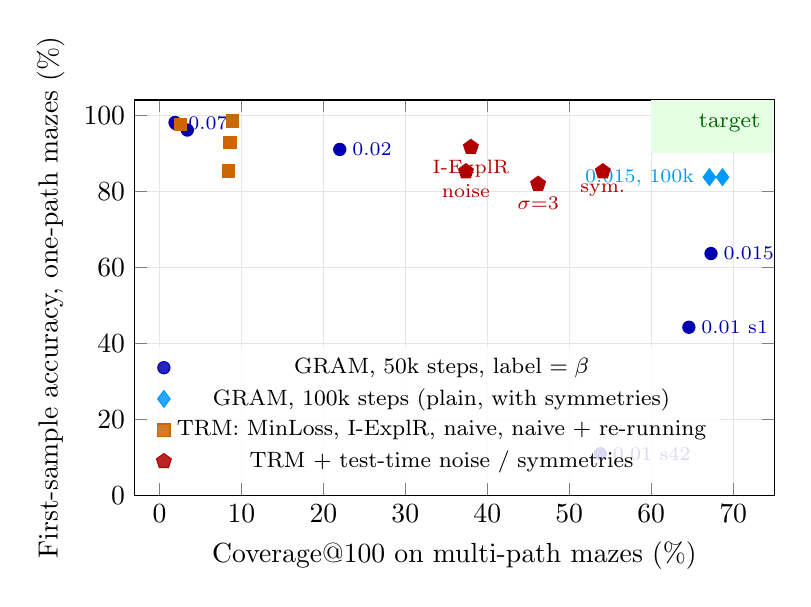
\begin{tikzpicture}
\begin{axis}[
  width=0.8\linewidth, height=6.6cm,
  xlabel={Coverage@100 on multi-path mazes (\%)},
  ylabel={First-sample accuracy, \onepath{} mazes (\%)},
  xmin=-3, xmax=75, ymin=0, ymax=104,
  grid=major, grid style={gray!20},
  legend style={at={(0.02,0.03)},anchor=south west,font=\footnotesize,draw=none,fill=white,fill opacity=0.85,text opacity=1},
]
\fill[green!10] (axis cs:60,90) rectangle (axis cs:75,104);
\node[font=\footnotesize,green!40!black,anchor=north east] at (axis cs:74.5,103) {target};
\addplot[only marks, mark=*, mark size=2.2pt, blue!70!black,
  nodes near coords, point meta=explicit symbolic,
  every node near coord/.style={font=\scriptsize, anchor=west, xshift=1pt}]
  coordinates {(2.0,97.8)[0.07] (1.9,98.1)[] (3.4,96.1)[] (22.0,91.0)[0.02] (67.3,63.6)[0.015] (64.6,44.2)[0.01 s1] (53.8,10.9)[0.01 s42]};
\addlegendentry{GRAM, 50k steps, label $=\beta$}
\addplot[only marks, mark=diamond*, mark size=3pt, blue!40!cyan,
  nodes near coords, point meta=explicit symbolic,
  every node near coord/.style={font=\scriptsize, anchor=east, xshift=-2pt}]
  coordinates {(67.1,83.7)[0.015, 100k] (68.7,83.7)[]};
\addlegendentry{GRAM, 100k steps (plain, with symmetries)}
\addplot[only marks, mark=square*, mark size=2.2pt, orange!80!black] coordinates {(8.4,85.3) (8.6,92.8) (2.6,97.6) (8.9,98.5)};
\addlegendentry{TRM: MinLoss, I-ExplR, naive, naive + re-running}
\addplot[only marks, mark=pentagon*, mark size=2.8pt, red!70!black,
  nodes near coords, point meta=explicit symbolic,
  every node near coord/.style={font=\scriptsize, anchor=north, yshift=-1pt}]
  coordinates {(37.4,85.2)[noise] (46.2,81.9)[$\sigma{=}3$] (54.1,85.2)[sym.] (38.0,91.6)[I-ExplR]};
\addlegendentry{TRM + test-time noise / symmetries}
\end{axis}
\end{tikzpicture}
\caption{Reliability against coverage on mazes. Longer training moves GRAM close to the target region; test-time
perturbation moves deterministic TRMs (MinLoss unless labelled) most of the way across.}
\label{fig:tradeoff}
\end{figure}

\subsection{Naive training fails at decoding, not at learning}
\label{sec:decoding}

\paragraph{What one pass holds.} The common explanation for naive training's failure is that the model averages the
solutions, so cells where the solutions disagree get split probability~\cite{nandwani2021oneofmany}. Measuring the
per-cell probabilities of naive TRM shows something else.
\begin{itemize}
  \item \textbf{N-Queens: one confident choice per row, not a blend.} On rows where the solutions put their queen in
  different columns, 95.5\% have a single column with $\geq$99\% of the row's queen probability. But the row's total
  queen probability is low (0.45 on unique-solution boards, 0.26 at 5--19 solutions, 0.05 at 20+), below the 0.5
  needed by a per-cell readout. Reading each row's most likely column from the same single pass gives 66.7\% valid
  boards instead of 1.0\% (Random: 73.3\% instead of 23\%). The remaining invalid boards combine rows that are each
  confident, but follow different solutions.
  \item \textbf{Mazes: abstaining at forks.} Naive TRM is confident on cells every shortest path uses (0.96), but at
  91\% of forks it puts less than 0.05 probability on every continuation (MinLoss: 61\%). The one-shot readout then
  marks a broken path.
  \item \textbf{The choice is made early.} At 94--99\% of maze forks, the continuation preferred after the first
  supervision step is the final one; on N-Queens 64\% of choices are fixed after step 1 and 90\% after step 2. This is
  why extra recursion at test time (32 instead of 16 steps) and noise injected after the first step changed nothing
  for any model.
\end{itemize}

\begin{table}[h]
\centering\small
\begin{tabular}{@{}llccccc@{}}
\toprule
& Decoding & Passes & all & one solution & several & by solutions \\
\midrule
\multirow{4}{*}{\shortstack[l]{Mazes,\\naive TRM}} & one shot (cell readout) & 1.00 & 37.2 & 97.6 & 7.0 & -- \\
& walk, one pass & 1.00 & 67.7 & 97.6 & 52.7 & 256+ paths: 43.6 \\
& walk, re-run when unsure & 2.27 & 90.5 & 97.6 & 86.9 & 256+ paths: 91.2 \\
& walk, re-run every step & 14.85 & \textbf{99.4} & \textbf{98.5} & \textbf{99.8} & all bins $\geq$98.5 \\
\midrule
\multirow{4}{*}{\shortstack[l]{N-Queens,\\naive TRM}} & one shot (cell readout) & 1 & 1.0 & -- & -- & \\
& row readout, one pass & 1 & 66.7 & 55 & -- & 10--19 sol.: 39.9 \\
& commit, re-run when unsure & 1.06 & 67.0 & -- & -- & \\
& commit, re-run every step & $\leq$9 & 77.9 & 62.7 & -- & 10--19 sol.: 92.1 \\
\midrule
\multicolumn{2}{@{}l}{Mazes, MinLoss / I-ExplR, walk when unsure} & 1.01 & 95.7 / 97.2 & 89.4 / 94.0 & 98.9 / 98.9 & \\
\multicolumn{2}{@{}l}{Mazes, GRAM 100k, majority of 20 samples} & 20 & 98.7 & 97.2 & 99.5 & \\
\multicolumn{2}{@{}l}{N-Queens, MinLoss / GRAM, one shot} & 1 & 96.5 / 91.0 & 93 / 82.8 & & \\
\bottomrule
\end{tabular}
\caption{Decoding naive TRM one decision at a time (seed 42). ``Re-run when unsure'' re-runs the model only when the
next decision's normalised probability is below 0.99. On N-Queens every run places at most 9 queens.}
\label{tab:ladder}
\end{table}

\paragraph{Committing and re-running.} Table~\ref{tab:ladder} decodes naive TRM sequentially. Three observations.
\begin{itemize}
  \item \textbf{Re-running is what matters, not reading out one decision at a time.} On mazes a walk that never
  re-runs the model reaches 67.7\%; re-running at every step reaches 99.4\%, with all path-count bins at 98.5\% or
  above. Random TRM, trained on a single arbitrary path per maze, gains as much as naive TRM (35.1\% $\to$ 89.9\%), so
  the gain does not depend on having learned how the solutions are distributed.
  \item \textbf{Confidence does not show where to re-run.} Re-running only when the model is unsure helps on mazes
  (90.5\%), where the model abstains at forks, but not on N-Queens (67.0\% at 1.06 passes), where the model is
  confidently inconsistent: the mixed-up rows each look certain.
  \item \textbf{A crossover on mazes.} Naive TRM with re-running (99.4\%, one answer, 15 passes) beats MinLoss and
  I-ExplR with walk decoding (95.7\%, 97.2\%) and matches GRAM with majority voting at similar compute (98.0\% at 10
  samples, 98.7\% at 20; 99.4\% at 20 with symmetric views). Without a decoding change, naive TRM is the worst of
  these models. A caveat: walking also shrinks the maze, so the other models may gain from re-running too. This is
  the next experiment.
\end{itemize}
On N-Queens, re-running fixes the ambiguous queries (10--19 solutions: 39.9\% $\to$ 92.1\%) but not the unique ones
(62.7\%, against 93\% for MinLoss). This is the second kind of error.

\subsection{Two kinds of error}

\begin{table}[h]
\centering\small
\begin{tabular}{@{}lcccccc@{}}
\toprule
& & \multicolumn{3}{c}{Share of invalid answers} & \multicolumn{2}{c}{Invalid on mazes with} \\
\cmidrule(lr){3-5}\cmidrule(l){6-7}
Maze walk decoding & Invalid & detour & stuck & wrong turn at fork & 1 path & 256+ paths \\
\midrule
naive TRM, one pass & 32.3 & 10.7 & 89.3 & 44.4 & 2.4 & 56.4 \\
naive TRM, re-run when unsure & 9.6 & 47.1 & 52.9 & 62.3 & 2.4 & 8.8 \\
naive TRM, re-run every step & 0.6 & 91.7 & 8.3 & 0.0 & 1.5 & 0.0 \\
TRM + MinLoss & 4.3 & 68.6 & 31.4 & 0.0 & 10.6 & 0.0 \\
TRM + I-ExplR & 2.8 & 76.4 & 23.6 & 0.0 & 6.0 & 0.0 \\
GRAM, $\beta=0.015$, 100k & 8.4 & 90.5 & 9.5 & 5.7 & 15.2 & 1.6 \\
\bottomrule
\end{tabular}
\caption{Failed maze walks. Detour: reached the goal by a longer route. Stuck: did not reach the goal. Wrong turn at
a fork: the first cell off every shortest path was entered from a cell with several shortest continuations.}
\label{tab:failures}
\end{table}

Table~\ref{tab:failures} separates the errors. Naive TRM's walk errors are ambiguity errors: they happen on mazes with
many paths, mostly as wrong turns at forks, and re-running at every step removes them. MinLoss and I-ExplR never take
a wrong turn at a fork; their errors are detours on \onepath{} mazes, where they are worse than naive TRM (MinLoss
85.3\% vs.\ 97.6\% one-shot). GRAM's errors look the same. These are solver errors, and the training objective is
what moves them, in a direction that depends on the domain: on mazes naive training is the best solver on unique
inputs (97.6--98.5\%, against 85--93\% for the one-of-many objectives and 84\% for GRAM), on N-Queens the worst
(55--63\% against 93\%). The 1oML objectives do two things at once: they remove ambiguity from the training signal,
which decoding can also do, and they change how well the model solves unique inputs, which decoding cannot.

\subsection{Diversity without a latent variable}
\label{sec:diversity}

Since a deterministic model's choice is fixed in the first recursion steps (Section~\ref{sec:decoding}), its initial
latent state is a natural place to inject randomness. With 4 noise draws, naive TRM still returns the same answer on
92--95\% of inputs (its choice is set by the input), but MinLoss only on 27--54\%. We therefore sampled 100 answers per
input from MinLoss, I-ExplR and Unique with noise on the initial state, alone or combined with the 8 board symmetries.

\begin{table}[h]
\centering\small
\begin{tabular}{@{}lcccccc@{}}
\toprule
& \multicolumn{3}{c}{Majority vote} & \multicolumn{2}{c}{Coverage} & Hidden constr. \\
\cmidrule(lr){2-4}\cmidrule(lr){5-6}
N-Queens, 100 samples & @1 & @5 & @100 & @5 & @100 & $f<0.1$, @100 \\
\midrule
TRM + MinLoss, deterministic & 96.5 & -- & -- & $\approx$34 & $\approx$34 & 7.6 \\
TRM + MinLoss, noise & \textbf{96.6} & 97.3 & 97.8 & 67.9 & 96.4 & 85.3 \\
TRM + MinLoss, noise + symmetries & \textbf{96.6} & \textbf{98.6} & 99.2 & 77.6 & 99.5 & 95.6 \\
TRM + I-ExplR, noise + symmetries & 92.7 & 97.8 & 99.0 & 76.8 & 99.8 & 98.1 \\
TRM + Unique, noise + symmetries & 81.0 & 86.2 & 89.1 & 70.9 & 98.4 & 88.0 \\
GRAM & 91.0 & \textbf{98.6} & \textbf{100.0} & \textbf{78.0} & \textbf{99.9} & \textbf{99.2} \\
GRAM + symmetries & 91.0 & \textbf{98.7} & \textbf{100.0} & \textbf{78.9} & \textbf{99.9} & \textbf{99.2} \\
\bottomrule
\end{tabular}
\caption{N-Queens with test-time diversity ($\sigma=1$, seed 42). Every model finds a valid answer within 100 samples
on all boards.}
\label{tab:div-nqueens}
\end{table}

\begin{table}[h]
\centering\small
\begin{tabular}{@{}lccccccc@{}}
\toprule
& \multicolumn{3}{c}{Majority vote} & Coverage & & Distinct & best-Q \\
\cmidrule(lr){2-4}
Mazes, 100 samples & @1 & @10 & @100 & @100 & Evenness & paths & @100 \\
\midrule
TRM + MinLoss, deterministic & 94.0 & -- & -- & 8.4 & -- & 1.0 & -- \\
TRM + MinLoss, noise & 94.0 & 94.4 & 94.4 & 37.4 & 6.86 & 16.6 & 96.1 \\
TRM + MinLoss, noise $\sigma=3$ & 92.8 & 94.2 & 94.5 & 46.2 & 5.77 & 26.1 & 96.2 \\
TRM + MinLoss, noise + symmetries & 94.0 & 97.5 & 97.5 & 54.1 & 4.04 & 28.7 & 98.2 \\
TRM + I-ExplR, noise + symmetries & \textbf{96.4} & \textbf{98.5} & 98.8 & 38.0 & 4.88 & 14.3 & \textbf{99.3} \\
TRM naive, noise + symmetries & 37.1 & 38.8 & 39.6 & 9.0 & 4.94 & 1.7 & 43.8 \\
GRAM, 100k steps & 91.3 & 97.8 & 99.1 & 67.1 & 2.45 & 41.0 & 76.7 \\
GRAM, 100k steps + symmetries & 91.3 & 98.0 & \textbf{99.7} & \textbf{68.7} & \textbf{1.59} & \textbf{42.7} & 86.2 \\
\bottomrule
\end{tabular}
\caption{Mazes with test-time diversity (seed 42). Distinct paths per multi-path maze among valid samples; a uniform
sampler drawing as many valid paths finds about 44. best-Q: the sample with the highest halting logit among 100.}
\label{tab:div-maze}
\end{table}

Tables~\ref{tab:div-nqueens} and~\ref{tab:div-maze} show the results.
\begin{itemize}
  \item \textbf{On N-Queens, a deterministic model matches GRAM.} MinLoss with noise and symmetries covers 99.5\% of
  the solutions in 100 samples (GRAM 99.9\%), equals GRAM's majority vote at 5 samples (98.6\%), and has a better first
  sample (96.6\% vs.\ 91.0\%). GRAM still wins at 10 or more votes (99.8\% vs.\ 98.8\%) and on the rarest hidden
  constraints (99.2\% vs.\ 95.6\%). The reason is visible on unique-solution boards: GRAM's wrong samples are scattered
  (17 distinct answers per board), so voting removes them; MinLoss's are systematic (1.8 distinct answers), so voting
  plateaus at 98.5\%.
  \item \textbf{On mazes, it closes most of the gap, not all.} Coverage rises from 8\% to 54\% (GRAM 67--69\%), but
  paths are drawn about $2.5\times$ less evenly. Larger noise buys coverage at the cost of first-sample accuracy
  ($\sigma=3$). The number of shortest paths, up to 924, is the likely difference: perturbing the starting state
  selects among a few tie-breaking outcomes rather than spreading over hundreds of paths.
  \item \textbf{Symmetric views are a free improvement for every model.} They add coverage and evenness to GRAM too
  (evenness 2.45 $\to$ 1.59) and raise voted accuracy, including on \onepath{} mazes (MinLoss 85\% $\to$ 94\%).
  \item \textbf{Naive TRM gains nothing.} Its one-shot readout is broken, so its samples are wrong in new ways; it needs
  the decoding of Section~\ref{sec:decoding} first.
\end{itemize}

\paragraph{Choosing among samples without a checker (H5).} The halting head predicts whether the current answer is
correct. For deterministic TRMs sampled with noise and symmetries, picking the sample it rates highest improves with
the number of samples (I-ExplR 96.4\% $\to$ 99.3\% at 100, MinLoss 94.0\% $\to$ 98.2\%), better than majority vote. For
GRAM it gets worse as samples are added (91.3\% $\to$ 76.7\% at 100; 200k-step continuation 43.1\%), presumably
because its halting head is trained on predictions made with posterior latents and is fooled by unusual prior
samples. I-ExplR with symmetries and halting-head selection (99.3\%) is the best verifier-free result on mazes after
naive TRM with re-running and GRAM with 100 votes over symmetric views (99.7\%).

\section{What the evidence supports so far}

\begin{itemize}
  \item \textbf{D1 is supported on both tasks.} Naive training fails by inconsistent or missing commitments in one
  parallel pass, not by averaging, and committing with re-running removes ambiguity errors. On mazes this makes the
  naive model the best single-answer model; on N-Queens it does not, because of solver errors.
  \item \textbf{D2 is supported on mazes and consistent with N-Queens.} Ambiguity errors and solver errors are
  distinct, and the training objective mainly moves the second.
  \item \textbf{D3 is supported on both tasks.} Test-time perturbation of the initial state gives deterministic
  models diversity, enough to match GRAM where there are few solutions per input and most of it where there are
  hundreds.
  \item \textbf{GRAM's distinctive strength is calibrated diversity}: the most even coverage, scattered errors that
  voting removes, and the best results on rare hidden constraints. Its first sample is not its strength, and its
  halting head cannot select among its own samples.
\end{itemize}
All of these are single-seed results, except where a second seed is reported.

\section{Plan}
\label{sec:plan}

Each experiment is tied to a question, a baseline and a decision rule fixed in advance.

\begin{table}[h]
\centering\small
\begin{tabular}{@{}p{0.6cm}p{4.3cm}p{3.0cm}p{6.2cm}@{}}
\toprule
& Experiment & Baseline & Decision rule \\
\midrule
D1 & Re-running at every step for MinLoss, I-ExplR and GRAM 100k, mazes and N-Queens & naive TRM with re-running
& If they stay below naive TRM on mazes (99.4\%), the crossover holds: decoding, not the objective, handles ambiguity.
If they rise above it, re-running also fixes solver errors, and the crossover claim is withdrawn \\
D1 & Mode mixing in naive N-Queens failures (analysis only) & -- & Share of failed boards whose rows each belong to some
solution: high supports ``confidently inconsistent'' \\
all & Second seed: naive TRM decoding on both tasks; GRAM $\beta=0.015$ 100k from scratch & seed 42 & Claims stand if
the seed-1 numbers are within 5 points \\
D3 & Halting-head selection on N-Queens samples (analysis only) & majority vote & Same direction as mazes (helps TRM,
hurts GRAM) \\
all & Third task: Sudoku with several solutions & both tasks & D1--D3 replicate \\
\bottomrule
\end{tabular}
\caption{Next experiments.}
\label{tab:plan}
\end{table}

\section{Risks and limitations}

\begin{itemize}
  \item \textbf{Seeds.} Most results are single-seed; N-Queens shows up to 8 points of seed variance between seeds.
  \item \textbf{Compute is not matched across decoding methods.} Re-running at every step costs about 15 passes per
  maze, and comparisons are only fair against sampling methods at similar cost, which we report.
  \item \textbf{Walking shrinks the maze.} Part of the gain from re-running may come from easier subproblems rather
  than from resolving ambiguity; the planned run on the 1oML models separates the two.
  \item \textbf{Training protocol.} Learning rate is constant; continuing finished runs degraded every model, so we
  compare only runs trained from scratch.
  \item \textbf{Memorisation on N-Queens.} Test answers appear in training; maze results do not have this problem.
  \item \textbf{Synthetic tasks.} The link to language-model reasoning is by analogy.
\end{itemize}

\begin{thebibliography}{99}\small
\bibitem{baek2026gram} J.~Baek, M.~Jo, M.~Kim, M.~Ren, Y.~Bengio, and S.~Ahn. Generative recursive reasoning.
\emph{arXiv:2605.19376}, 2026.
\bibitem{jolicoeur2025trm} A.~Jolicoeur-Martineau. Less is more: Recursive reasoning with tiny networks.
\emph{arXiv:2510.04871}, 2025.
\bibitem{wang2025hrm} G.~Wang et al. Hierarchical reasoning model. \emph{arXiv:2506.21734}, 2025.
\bibitem{nandwani2021oneofmany} Y.~Nandwani, D.~Jindal, Mausam, and P.~Singla. Neural learning of one-of-many
solutions for combinatorial problems in structured output spaces. In \emph{ICLR}, 2021.
\bibitem{gu2018nat} J.~Gu, J.~Bradbury, C.~Xiong, V.~O.~K.~Li, and R.~Socher. Non-autoregressive neural machine
translation. In \emph{ICLR}, 2018.
\bibitem{kim2025ordering} J.~Kim, K.~Shah, V.~Kontonis, S.~Kakade, and S.~Chen. Train for the worst, plan for the
best: Understanding token ordering in masked diffusions. In \emph{ICML}, 2025.
\bibitem{brown2024monkeys} B.~Brown, J.~Juravsky, R.~Ehrlich, R.~Clark, Q.~V.~Le, C.~R\'e, and A.~Mirhoseini. Large
language monkeys: Scaling inference compute with repeated sampling. \emph{arXiv:2407.21787}, 2024.
\bibitem{wang2023selfconsistency} X.~Wang, J.~Wei, D.~Schuurmans, Q.~Le, E.~Chi, S.~Narang, A.~Chowdhery, and
D.~Zhou. Self-consistency improves chain of thought reasoning in language models. In \emph{ICLR}, 2023.
\bibitem{cobbe2021verifiers} K.~Cobbe, V.~Kosaraju, M.~Bavarian, M.~Chen, H.~Jun, L.~Kaiser, M.~Plappert,
J.~Tworek, J.~Hilton, R.~Nakano, C.~Hesse, and J.~Schulman. Training verifiers to solve math word problems.
\emph{arXiv:2110.14168}, 2021.
\bibitem{snell2024scaling} C.~Snell, J.~Lee, K.~Xu, and A.~Kumar. Scaling LLM test-time compute optimally can be more
effective than scaling model parameters. \emph{arXiv:2408.03314}, 2024.
\bibitem{wen2025rlvr} X.~Wen et al. Reinforcement learning with verifiable rewards implicitly incentivizes correct
reasoning in base LLMs. \emph{arXiv:2506.14245}, 2025.
\bibitem{yue2025rl} Y.~Yue et al. Does reinforcement learning really incentivize reasoning capacity in LLMs beyond
the base model? \emph{arXiv:2504.13837}, 2025.
\end{thebibliography}

\end{document}
